\section{The Repair Decision: Diagnosing When Anti-Smoothing Helps}
\label{sec:law}

The oracle gap is one branch of a repair decision; Section~\ref{sec:regionfocal} completes the tree with the level-lag regime. Cells are routed by the residual's dominant bias type, measured by the signed residual effect size $|\mathbb{E}[r]|/\mathrm{std}(r)$ over the test windows: dispersion-dominated cells are gated by the oracle gap here, while lag-dominated cells are analyzed in Section~\ref{sec:regionfocal}. The two regimes separate bimodally on every cell we tested---at most $0.052$ on the dispersion cells of Table~\ref{tab:law} and at least $0.110$ on the lag cells of Section~\ref{sec:regionfocal}---so no conclusion depends on the routing threshold. We evaluate the pairing of the oracle gap with \rfc~(Section~\ref{sec:regionfocal}) on sixteen dispersion-regime dataset-backbone cells, eleven across nine datasets in Table~\ref{tab:law} and five across backbones in Appendix~\ref{app:matrix}. The sign of the gap predicts the direction of the intervention's effect on fifteen of the sixteen cells, counting changes within $\pm 0.5\%$ as neutral; the single exception is analyzed below. The two largest gaps give the largest improvements and all non-positive gaps give neutral or negative effects; the magnitude relation is monotone but coarse, and we treat the sign, not the magnitude, as the diagnostic's decision variable. Under a sign-symmetric null the probability of fifteen or more sign-consistent cells out of sixteen is below $3 \times 10^{-4}$, so the gate is a statistical regularity, not a coincidence.

\begin{table}[t]
  \footnotesize
  \caption{The oracle gap predicts the effect of dispersion-targeting repair (\rfc). Negative relative MSE change is better. Multi-seed cells report the mean over seeds 2021--2023, single-seed cells use seed 2021; Traffic cells use $\alpha{=}0.5$ (the development-selected value, Table~\ref{tab:main}) and all others $\alpha{=}1$. $\dagger$: descriptor-head variant.}
  \label{tab:law}
  \centering
  \begin{tabular}{llccc}
    \toprule
    Dataset & Backbone & Oracle gap & $\Delta$MSE (\%) & Prediction \\
    \midrule
    Electricity & PatchTST & $+0.030$ & $-2.3$ & \checkmark \\
    Traffic & PatchTST & $+0.027$ & $-1.0$ & \checkmark \\
    Traffic & iTransformer & $-0.023$ & $+4.4$ & \checkmark \\
    Traffic & FreTS & $+0.013$ & $+0.9$ & $\times$ \\
    solar/H & PatchTST & $+0.017$ & $-2.5$ & \checkmark \\
    SWaT & PatchTST & $+0.006$ & $+0.1$ & \checkmark \\
    bizitobs\_app. & PatchTST & $+0.009$ & $-1.7$ & \checkmark \\
    SZ\_TAXI & PatchTST & $-0.010$ & $+0.4$ & \checkmark \\
    ETTh1 & PatchTST & $-0.022$ & $+2.6$ & \checkmark \\
    ETTm1 & PatchTST & $-0.023$ & $-0.2$ & \checkmark \\
    Weather & PatchTST & $-0.058$ & $+2.5^{\dagger}$ & \checkmark \\
    \bottomrule
  \end{tabular}
\end{table}

The same law holds across five backbone families on Electricity (Appendix~\ref{app:matrix}, Table~\ref{tab:backbone}): the per-backbone gap, not the architecture family, orders the outcomes. The single sign-rule exception is FreTS on Traffic (gap $+0.013$, effect $+0.9 \pm 0.1\%$ across three seeds). It is diagnosable in advance: its under-shoot region does not dominate (rate $0.47$ versus $\ge 0.55$ on every improving dispersion cell), so up-weighting it barely shifts the gradient balance, and its signed bias concentrates in a minority of windows (top decile $59\%$, versus $11$--$18\%$ on the m4\_weekly cells); MAE fails there as well ($+4.7\%$). Both statistics are computable from a baseline run before any repair is trained (Appendix~\ref{app:negative}).

\subsection{A 665-cell audit of foundation models}
\label{sec:tsfmmap}

We extend the audit to thirteen zero-shot time-series foundation models, Chronos-Bolt at four scales (8M, 21M, 48M, 205M), Chronos-2, Sundial, Moirai-1.1 at two scales, Moirai-2.0, TimeMoE at two scales, Timer, and TiRex, on fifty dataset variants from GIFT-Eval \citep{gifteval} under the tail protocol. Figure~\ref{fig:map} summarizes the map.

\begin{figure}[t]
  \centering
  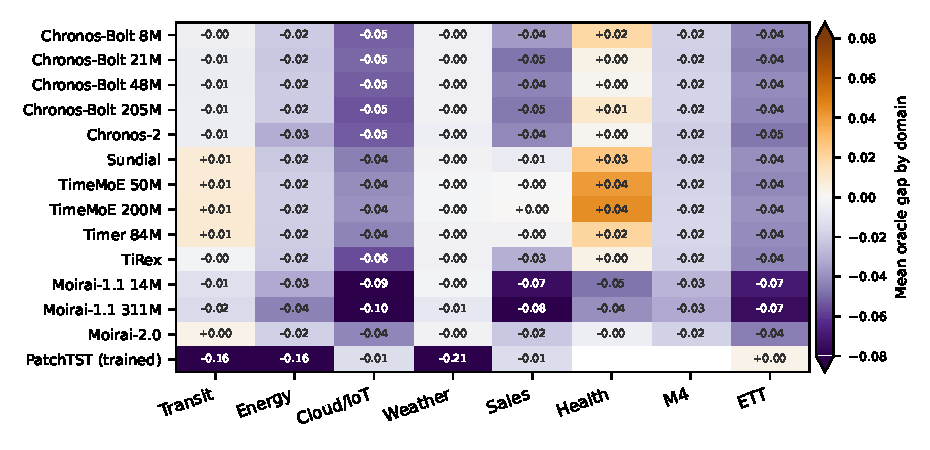
\includegraphics[width=\linewidth,height=3.4cm,keepaspectratio]{figures/fig_map_domain.pdf}
  \caption{Oracle gap aggregated by domain and model (means over the dataset variants within each domain). Positive gaps concentrate in transit and health series and are consistent across models; ETT variants are negative everywhere; the gap is flat across model scale. The two most positive single variants are SZ\_TAXI/15T ($+0.072$) and bizitobs\_application ($+0.067$); the full fifty-variant heatmap is in Appendix~\ref{app:matrix}.}
  \label{fig:map}
\end{figure}


\paragraph{The audit as a benchmark statement.}
The map quantifies benchmark saturation: all ETT variants are non-positive on every model we tested, so anti-smoothing research evaluated on ETT alone is measuring rational shrinkage, and the remaining exploitable structure concentrates in transit, energy, and event-driven series. Within each variant, a model's accuracy rank anti-correlates with its oracle gap (median Spearman $\rho = -0.49$ across fifty variants, Wilcoxon $p < 10^{-6}$): the better a model fits a dataset, the less repairable structure its residuals retain. The leading positive-gap datasets are the useful exceptions---on m4\_weekly ($\rho = +0.87$) and bizitobs\_application ($\rho = +0.52$), even the most accurate models leave measurable structure behind, which is precisely where repair methods should be developed and evaluated. We release the full matrix and the diagnostic code.
